\documentclass[12pt,a4paper]{article}

\usepackage[utf8]{inputenc}
\usepackage[spanish]{babel}
\usepackage{graphicx}
\usepackage{geometry}
\geometry{a4paper, margin=2.5cm}
\usepackage{xcolor}
\usepackage{listings}
\usepackage{booktabs}
\usepackage{amsmath}
\usepackage{subcaption}
\usepackage{float}
\usepackage[colorlinks=true, linkcolor=blue, urlcolor=blue]{hyperref}

\definecolor{codegreen}{rgb}{0,0.6,0}
\definecolor{codegray}{rgb}{0.5,0.5,0.5}
\definecolor{codepurple}{rgb}{0.58,0,0.82}
\definecolor{backcolour}{rgb}{0.95,0.95,0.92}

\lstdefinestyle{mystyle}{
    backgroundcolor=\color{backcolour},   
    commentstyle=\color{codegreen},
    keywordstyle=\color{magenta},
    numberstyle=\tiny\color{codegray},
    stringstyle=\color{codepurple},
    basicstyle=\ttfamily\footnotesize,
    breakatwhitespace=false,         
    breaklines=true,                 
    captionpos=b,                    
    keepspaces=true,                 
    numbers=left,                    
    numbersep=5pt,                  
    showspaces=false,                
    showstringspaces=false,
    showtabs=false,                  
    tabsize=2,
    literate={á}{{\'a}}1 {é}{{\'e}}1 {í}{{\'i}}1 {ó}{{\'o}}1 {ú}{{\'u}}1
             {Á}{{\'A}}1 {É}{{\'E}}1 {Í}{{\'I}}1 {Ó}{{\'O}}1 {Ú}{{\'U}}1
             {ñ}{{\~n}}1 {Ñ}{{\~N}}1
}
\lstset{style=mystyle}

\title{\Huge\textbf{PROYECTO ESP32} \\ \Large Movimiento Armónico Simple con Pantalla OLED \\ \vspace{0.5cm} \normalsize \textit{Simulación interactiva de MHS con visualización gráfica en tiempo real y control serial}}
\author{Msc. Néstor Fabio Montoya Palacios}
\date{2026 \\ \vspace{0.2cm} \small Plataforma: ESP32 Dev Module}

\begin{document}

\maketitle
\tableofcontents
\newpage

% ══════════════════════════════════════════════════════════════
\section{Introducción}
% ══════════════════════════════════════════════════════════════

Este documento describe el proyecto ``Movimiento Armónico Simple con Pantalla OLED'', una aplicación educativa que combina física y electrónica digital con el microcontrolador ESP32. El sistema simula y visualiza en tiempo real el \textbf{Movimiento Armónico Simple (MHS)} --- con opción de amortiguamiento --- sobre una pantalla OLED SSD1306 de 128$\times$64 píxeles conectada por I2C.

El usuario puede modificar interactivamente los parámetros de la onda (amplitud, frecuencia, fase y coeficiente de amortiguamiento) a través del \textbf{Monitor Serial} del Arduino IDE, observando instantáneamente el efecto sobre la gráfica dibujada en la pantalla OLED.

El proyecto introduce conceptos fundamentales de:
\begin{itemize}
    \item \textbf{Movimiento Armónico Simple (MHS)} y su ecuación matemática.
    \item \textbf{Oscilaciones amortiguadas} con decaimiento exponencial.
    \item \textbf{Comunicación I2C} entre el ESP32 y la pantalla OLED.
    \item \textbf{Renderizado gráfico en tiempo real} sobre displays de baja resolución.
    \item \textbf{Interfaz serial interactiva} para control de parámetros en tiempo de ejecución.
\end{itemize}

% ══════════════════════════════════════════════════════════════
\section{Objetivo del Proyecto}
% ══════════════════════════════════════════════════════════════

Implementar un simulador visual e interactivo de Movimiento Armónico Simple utilizando el microcontrolador ESP32 y una pantalla OLED SSD1306, demostrando:
\begin{itemize}
    \item La representación gráfica en tiempo real de funciones sinusoidales sobre un display OLED de 128$\times$64 píxeles.
    \item El control interactivo de los cuatro parámetros fundamentales del MHS: amplitud ($A$), frecuencia ($f$), fase ($\varphi$) y amortiguamiento ($\beta$).
    \item La comunicación I2C entre el ESP32 y periféricos mediante la librería Wire.
    \item El procesamiento de comandos textuales a través del puerto serial.
    \item La aplicación de conceptos de física (oscilaciones) en un contexto de sistemas embebidos.
\end{itemize}

% ══════════════════════════════════════════════════════════════
\section{Materiales Necesarios}
% ══════════════════════════════════════════════════════════════

\begin{table}[h!]
\centering
\begin{tabular}{cll}
\toprule
\textbf{Cant.} & \textbf{Componente} & \textbf{Especificación} \\
\midrule
1 & ESP32 Dev Module & Microcontrolador dual-core con Wi-Fi/Bluetooth \\
1 & Pantalla OLED SSD1306 & 128$\times$64 px, interfaz I2C, 0.96'' \\
1 & Placa de expansión ESP32 & Con borneras de tornillo (opcional) \\
1 & Protoboard & Placa de pruebas de 830 puntos \\
4 & Cables jumper & Hembra-hembra para conexión I2C \\
1 & Cable USB & Para programación y alimentación \\
\bottomrule
\end{tabular}
\caption{Lista de materiales del proyecto MHS}
\end{table}

% ══════════════════════════════════════════════════════════════
\section{Esquema de Conexión}
% ══════════════════════════════════════════════════════════════

El circuito es minimalista: únicamente se conecta la pantalla OLED SSD1306 al ESP32 mediante el bus I2C (4 cables). No se requieren componentes adicionales como resistencias ni sensores.

\begin{figure}[H]
\centering
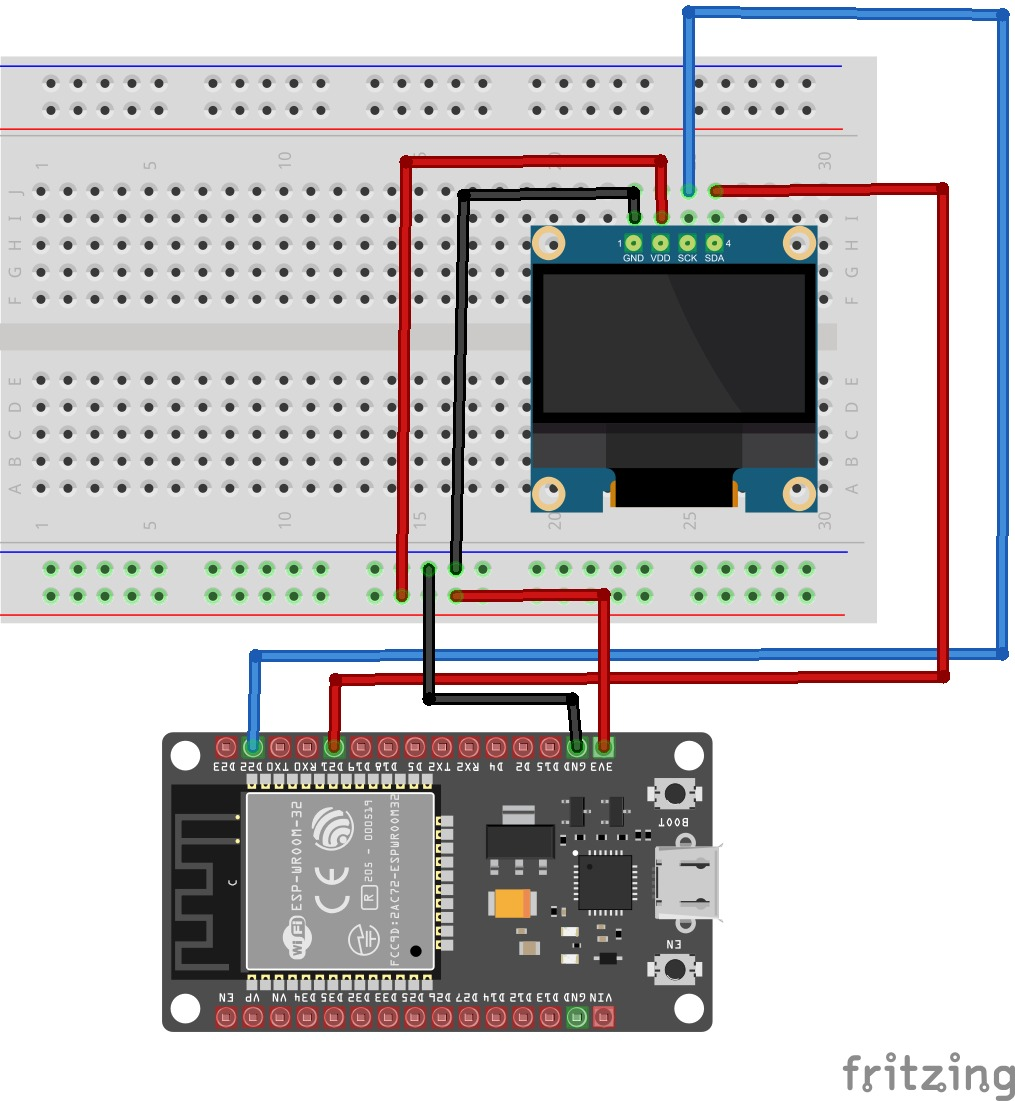
\includegraphics[width=0.75\textwidth]{../Esquemas/Armonico_esq.jpeg}
\caption{Esquema de conexión del circuito -- ESP32 con pantalla OLED SSD1306 (Fritzing)}
\label{fig:esquema}
\end{figure}

\subsection{Diagrama de Conexiones}

\begin{center}
\begin{tabular}{lll}
\toprule
\textbf{OLED SSD1306} & \textbf{Función} & \textbf{ESP32 GPIO} \\
\midrule
GND & Tierra & GND \\
VDD (VCC) & Alimentación & 3.3V \\
SCK (SCL) & Reloj I2C & GPIO22 (SCL) \\
SDA & Datos I2C & GPIO21 (SDA) \\
\bottomrule
\end{tabular}
\end{center}

\textbf{Nota:} El bus I2C del ESP32 utiliza por defecto GPIO21 (SDA) y GPIO22 (SCL). La pantalla OLED responde en la dirección I2C \texttt{0x3C}. Las líneas SDA y SCL del ESP32 ya incluyen resistencias pull-up internas, por lo que no es necesario añadir resistencias externas.

% ══════════════════════════════════════════════════════════════
\section{Fundamento Teórico}
% ══════════════════════════════════════════════════════════════

\subsection{Movimiento Armónico Simple (MHS)}

El MHS es un movimiento periódico en el que la posición de una partícula varía sinusoidalmente con el tiempo. La ecuación general es:

\begin{equation}
y(t) = A \sin(\omega t + \varphi)
\label{eq:mhs}
\end{equation}

donde:
\begin{itemize}
    \item $A$ es la \textbf{amplitud} (desplazamiento máximo desde el equilibrio).
    \item $\omega = 2\pi f$ es la \textbf{frecuencia angular} en rad/s.
    \item $f$ es la \textbf{frecuencia} en Hz (oscilaciones por segundo).
    \item $\varphi$ es la \textbf{fase inicial} en radianes.
    \item $T = 1/f$ es el \textbf{período} (tiempo de una oscilación completa).
\end{itemize}

\subsection{Oscilación Amortiguada}

En sistemas reales, la energía se disipa por fricción u otras fuerzas resistivas. La ecuación del MHS amortiguado introduce un factor de decaimiento exponencial:

\begin{equation}
y(t) = A \, e^{-\beta t} \sin(\omega t + \varphi)
\label{eq:amortiguado}
\end{equation}

donde $\beta \geq 0$ es el \textbf{coeficiente de amortiguamiento}:
\begin{itemize}
    \item $\beta = 0$: oscilación perpetua (MHS ideal, sin pérdidas).
    \item $0 < \beta < 1$: amortiguamiento leve (la onda se apaga gradualmente).
    \item $\beta \geq 1$: amortiguamiento fuerte (la onda se extingue rápidamente).
\end{itemize}

La envolvente $A \, e^{-\beta t}$ define la amplitud decreciente con el tiempo.

\subsection{Protocolo I2C}

I2C (\textit{Inter-Integrated Circuit}) es un protocolo de comunicación serie síncrono que utiliza dos líneas:
\begin{itemize}
    \item \textbf{SDA} (\textit{Serial Data}): línea bidireccional de datos.
    \item \textbf{SCL} (\textit{Serial Clock}): señal de reloj generada por el maestro (ESP32).
\end{itemize}

El ESP32 actúa como maestro y la pantalla OLED como esclavo en la dirección \texttt{0x3C}. La velocidad estándar es de 100\,kHz, aunque el ESP32 soporta hasta 400\,kHz (\textit{Fast Mode}).

% ══════════════════════════════════════════════════════════════
\section{Código Fuente}
% ══════════════════════════════════════════════════════════════

A continuación se presenta el código completo del proyecto.

\subsection{Código Completo}
\lstinputlisting[language=C++, title=Armonico.ino]{../Arduino/Armonico/Armonico.ino}

% ══════════════════════════════════════════════════════════════
\subsection{Análisis del Código}
% ══════════════════════════════════════════════════════════════

\subsubsection*{Librerías y Configuración de Hardware}

El programa utiliza tres librerías:
\begin{itemize}
    \item \textbf{Wire.h}: comunicación I2C con la pantalla OLED.
    \item \textbf{Adafruit\_GFX.h}: primitivas gráficas (píxeles, líneas, texto, círculos).
    \item \textbf{Adafruit\_SSD1306.h}: controlador específico del display SSD1306.
\end{itemize}

La pantalla se configura como 128$\times$64 píxeles en la dirección I2C \texttt{0x3C}, con los pines SDA=21 y SCL=22 del ESP32.

\subsubsection*{Parámetros del MHS}

Se definen cuatro variables globales que controlan la forma de onda:

\begin{center}
\begin{tabular}{lllll}
\toprule
\textbf{Variable} & \textbf{Comando} & \textbf{Rango} & \textbf{Default} & \textbf{Unidad} \\
\midrule
\texttt{amplitud} & \texttt{A:} & 1--28 & 25.0 & píxeles \\
\texttt{frecuencia} & \texttt{F:} & 0.1--10.0 & 1.0 & Hz \\
\texttt{fase} & \texttt{P:} & 0--6.28 & 0.0 & radianes \\
\texttt{amort} & \texttt{B:} & 0.0--2.0 & 0.0 & adimensional \\
\bottomrule
\end{tabular}
\end{center}

\subsubsection*{Función \texttt{setup()}}

\begin{enumerate}
    \item Inicia la comunicación serial a 115200 baudios.
    \item Inicializa el bus I2C con \texttt{Wire.begin(21, 22)}.
    \item Verifica la presencia de la pantalla OLED; si no se detecta, entra en un bucle infinito con mensaje de error.
    \item Muestra una pantalla de bienvenida ``MHS ESP32'' durante 1.5 segundos.
    \item Imprime en el Monitor Serial la tabla de comandos disponibles.
\end{enumerate}

\subsubsection*{Función \texttt{loop()}}

El bucle principal ejecuta dos tareas:
\begin{enumerate}
    \item \textbf{Procesamiento serial}: lee y parsea comandos del usuario (\texttt{A:}, \texttt{F:}, \texttt{P:}, \texttt{B:}, \texttt{R}, \texttt{?}).
    \item \textbf{Renderizado gráfico}: a $\sim$30 FPS (cada 33\,ms), redibuja la gráfica completa en la pantalla OLED.
\end{enumerate}

\subsubsection*{Función \texttt{calcY(t)} --- Cálculo de la Posición}

Esta función implementa directamente la ecuación~\ref{eq:amortiguado}:

\begin{verbatim}
float calcY(float t) {
    float omega = 2.0 * PI * frecuencia;
    float decay = exp(-amort * t);
    return amplitud * decay * sin(omega * t + fase);
}
\end{verbatim}

Calcula $\omega = 2\pi f$, el factor de decaimiento $e^{-\beta t}$, y retorna $y(t) = A \cdot e^{-\beta t} \cdot \sin(\omega t + \varphi)$.

\subsubsection*{Función \texttt{dibujarGrafica()} --- Renderizado OLED}

Esta función es el núcleo visual del proyecto:
\begin{enumerate}
    \item Limpia el buffer de la pantalla.
    \item Dibuja ejes cartesianos (horizontal en $y=32$, vertical en $x=4$).
    \item Muestra el título ``MHS'' y los parámetros $A$ y $f$ en la parte superior.
    \item Calcula una ventana temporal de 2 períodos: $\text{ventana} = 2/f$.
    \item Recorre 120 píxeles horizontales, calculando $y(t)$ para cada uno y conectando puntos consecutivos con segmentos verticales para suavizar la curva.
    \item Dibuja un marcador circular en la posición actual de la onda.
    \item Muestra el valor numérico $y$ actual y, si hay amortiguamiento, el coeficiente $\beta$.
\end{enumerate}

\subsubsection*{Función \texttt{procesarSerial()} --- Interfaz de Comandos}

Implementa un parser serial que acepta comandos con formato \texttt{LETRA:VALOR}:
\begin{itemize}
    \item \texttt{A:20} $\rightarrow$ cambia la amplitud a 20 píxeles.
    \item \texttt{F:2.5} $\rightarrow$ cambia la frecuencia a 2.5\,Hz.
    \item \texttt{P:1.57} $\rightarrow$ cambia la fase a $\pi/2$ rad.
    \item \texttt{B:0.5} $\rightarrow$ activa amortiguamiento con $\beta = 0.5$.
    \item \texttt{R} $\rightarrow$ resetea todos los parámetros a valores iniciales.
    \item \texttt{?} $\rightarrow$ muestra los parámetros actuales.
\end{itemize}

Cada comando incluye validación de rango y retroalimentación por serial.

% ══════════════════════════════════════════════════════════════
\section{Fotografías del Montaje}
% ══════════════════════════════════════════════════════════════

\subsection{Vista General del Proyecto}

\begin{figure}[H]
\centering
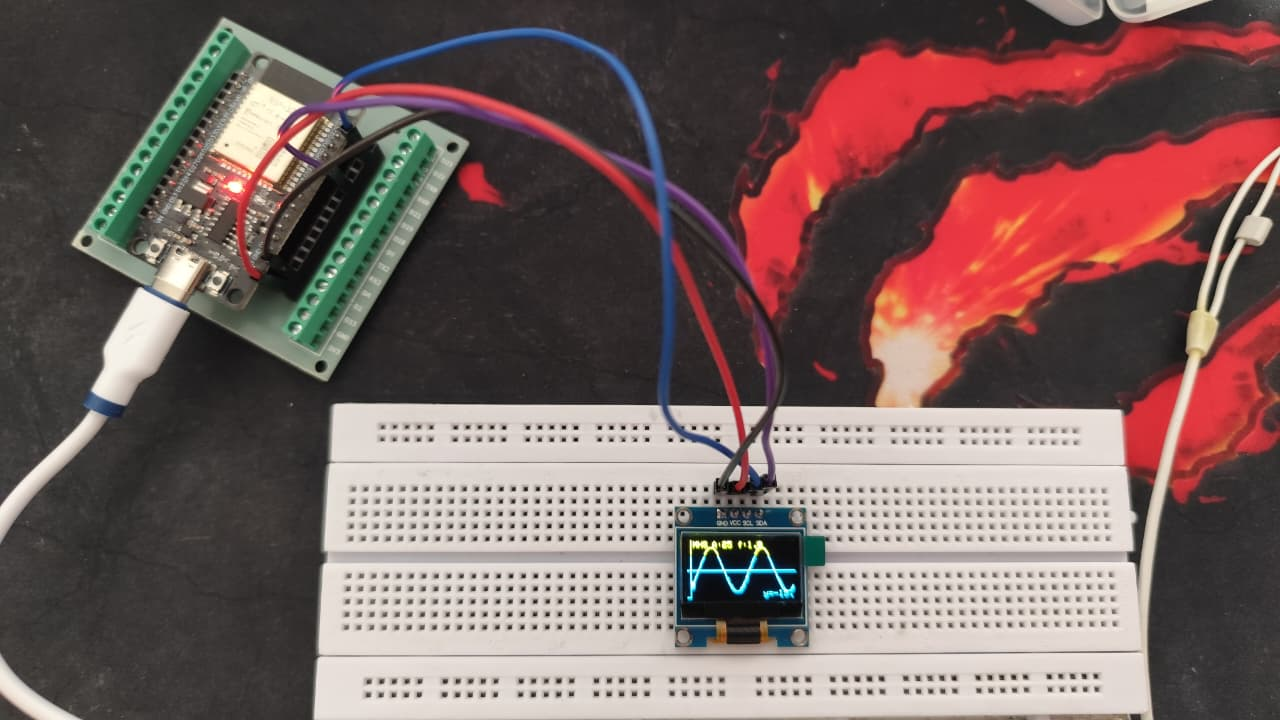
\includegraphics[width=0.75\textwidth]{../Imagenes/Armonico_imgs/Armonico_img13.jpeg}
\caption{Vista general del montaje: ESP32 en placa de expansión con borneras, conectado a la pantalla OLED SSD1306 montada en protoboard, mostrando una onda sinusoidal en tiempo real}
\label{fig:montaje_general}
\end{figure}

\subsection{Visualización de Ondas en la Pantalla OLED}

\begin{figure}[H]
\centering
\begin{subfigure}[b]{0.48\textwidth}
    \centering
    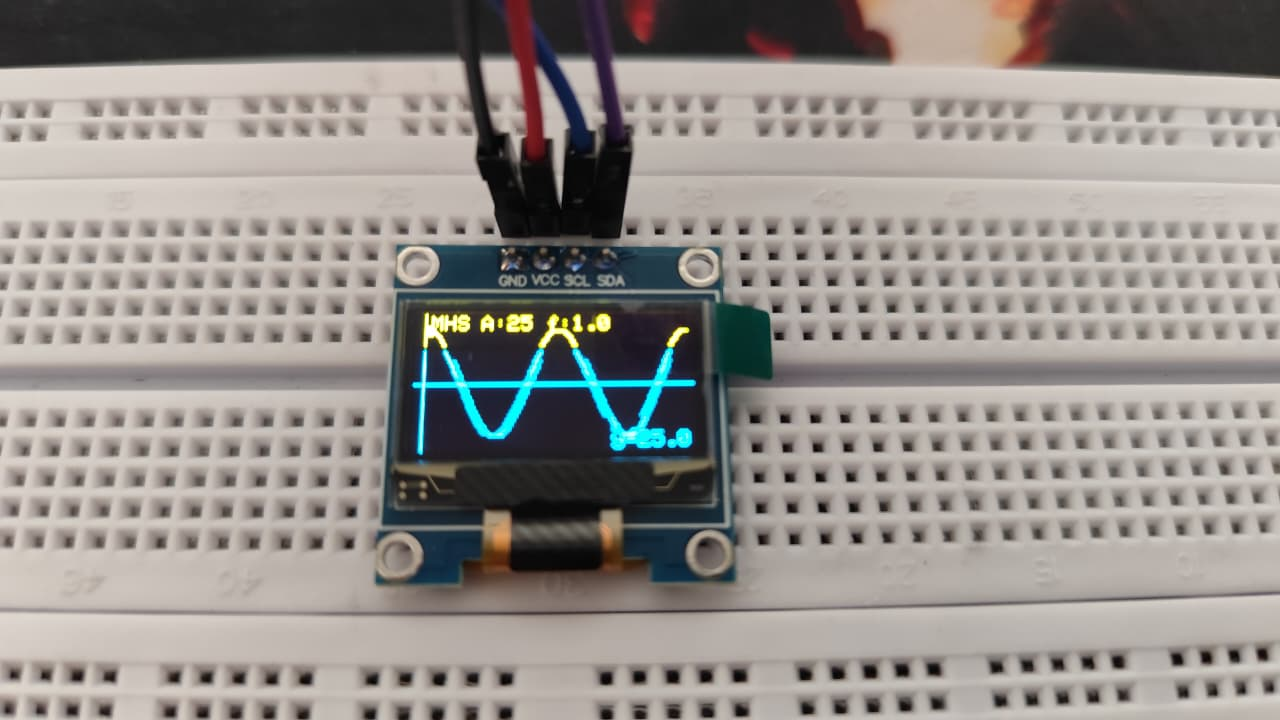
\includegraphics[width=\textwidth]{../Imagenes/Armonico_imgs/Armonico_img2.jpeg}
    \caption{MHS con $A=25$\,px, $f=1.0$\,Hz: onda sinusoidal completa de máxima amplitud}
    \label{fig:onda_default}
\end{subfigure}
\hfill
\begin{subfigure}[b]{0.48\textwidth}
    \centering
    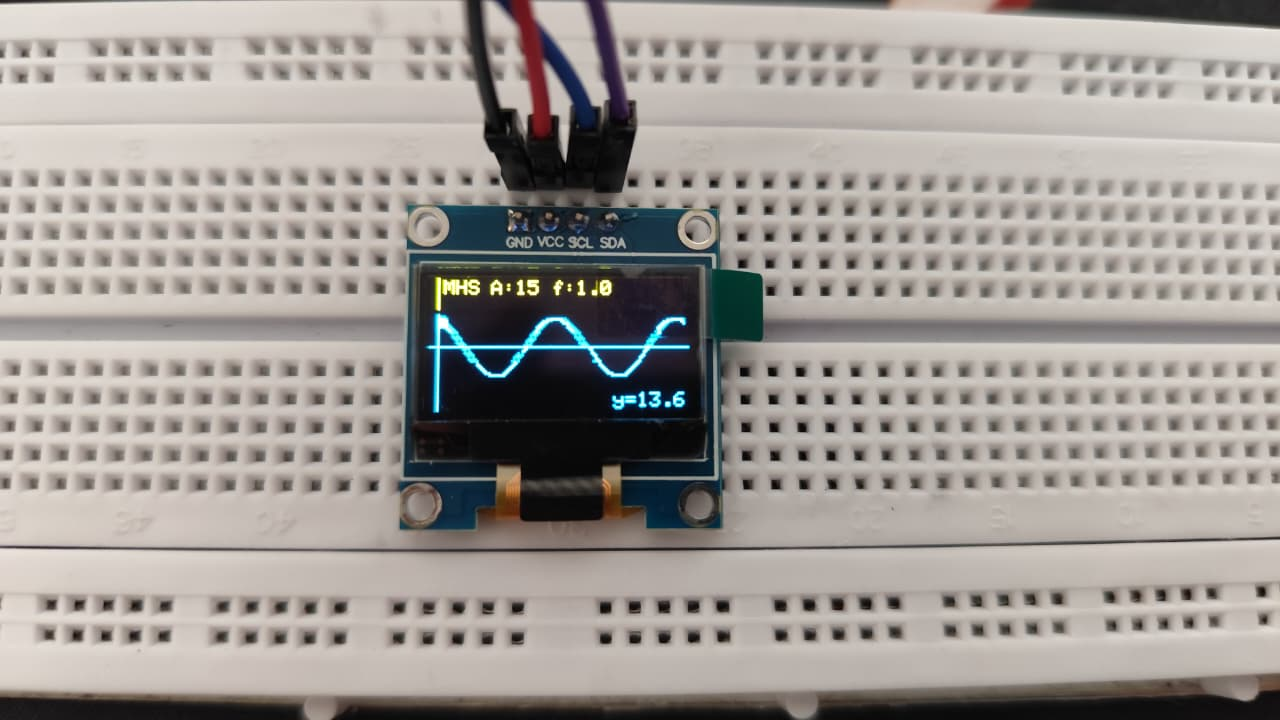
\includegraphics[width=\textwidth]{../Imagenes/Armonico_imgs/Armonico_img11.jpeg}
    \caption{MHS con $A=15$\,px, $f=1.0$\,Hz: amplitud reducida respecto al caso anterior}
    \label{fig:onda_a15}
\end{subfigure}
\caption{Efecto de la variación de amplitud sobre la forma de onda}
\label{fig:amplitudes}
\end{figure}

\begin{figure}[H]
\centering
\begin{subfigure}[b]{0.48\textwidth}
    \centering
    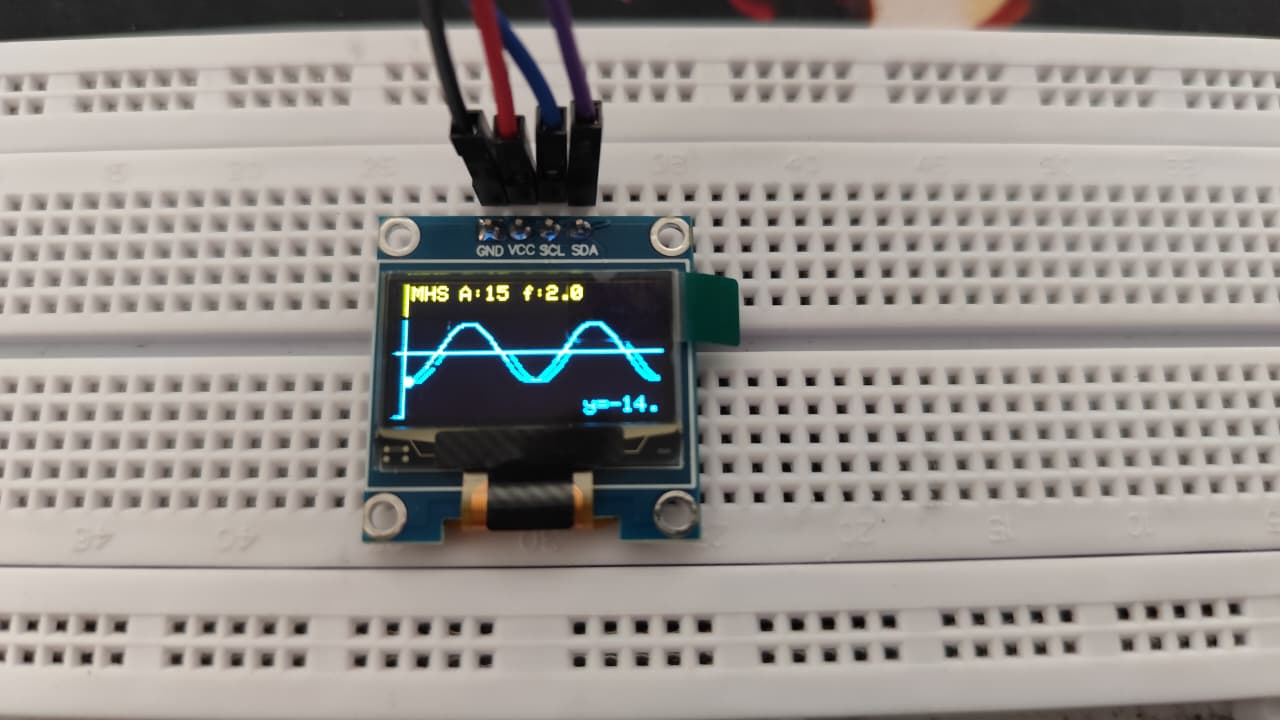
\includegraphics[width=\textwidth]{../Imagenes/Armonico_imgs/Armonico_img7.jpeg}
    \caption{MHS con $A=15$\,px, $f=2.0$\,Hz: frecuencia duplicada, más oscilaciones visibles}
    \label{fig:onda_f2}
\end{subfigure}
\hfill
\begin{subfigure}[b]{0.48\textwidth}
    \centering
    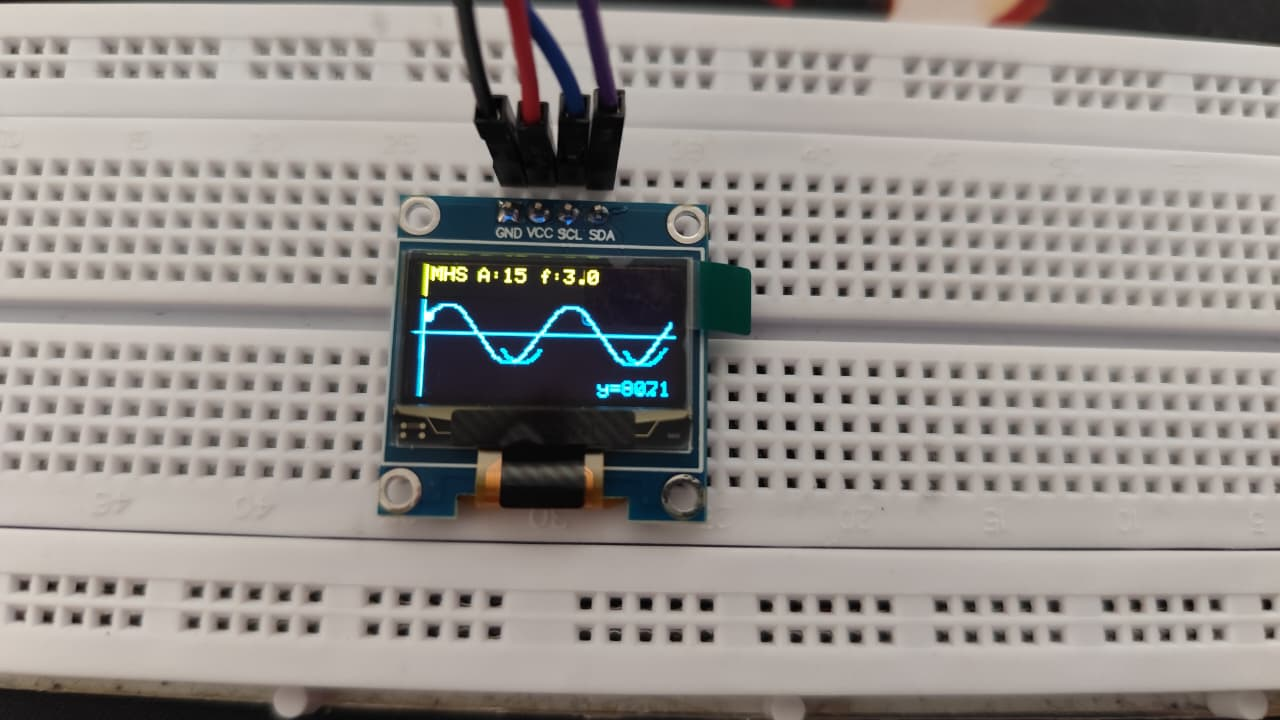
\includegraphics[width=\textwidth]{../Imagenes/Armonico_imgs/Armonico_img9.jpeg}
    \caption{MHS con $A=15$\,px, $f=3.0$\,Hz: frecuencia triplicada}
    \label{fig:onda_f3}
\end{subfigure}
\caption{Efecto de la variación de frecuencia sobre la forma de onda}
\label{fig:frecuencias}
\end{figure}

\begin{figure}[H]
\centering
\begin{subfigure}[b]{0.48\textwidth}
    \centering
    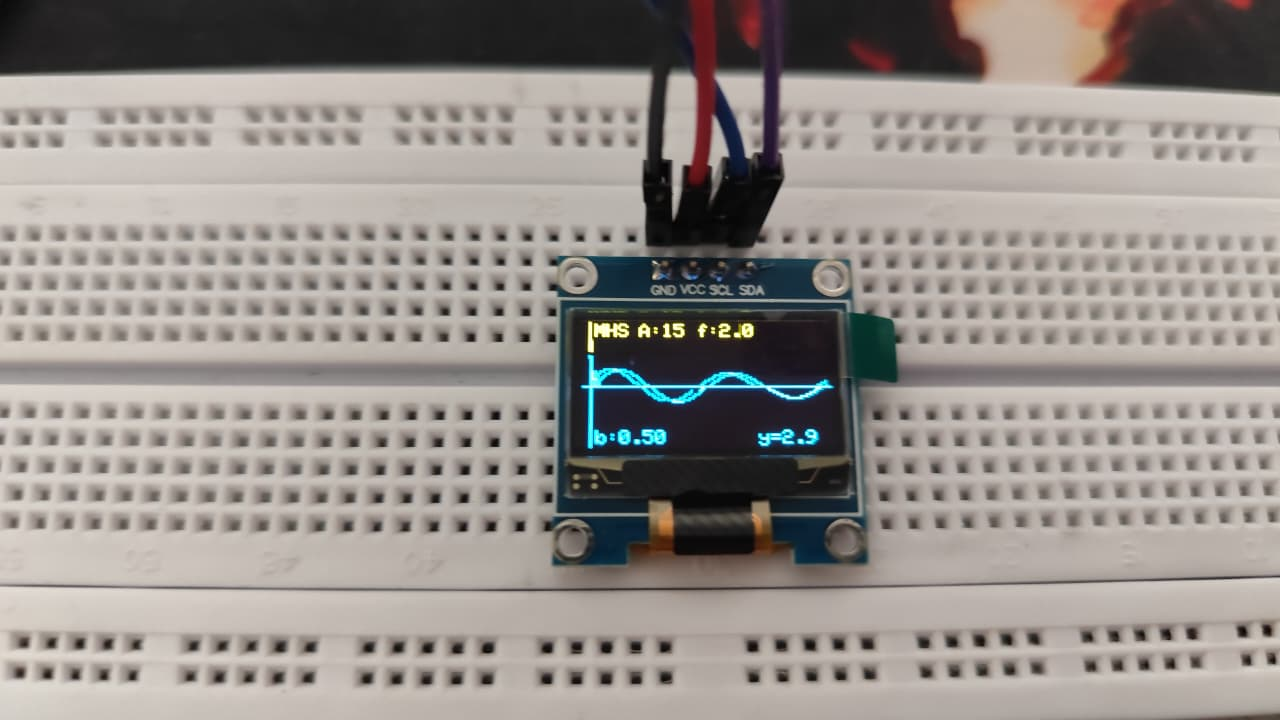
\includegraphics[width=\textwidth]{../Imagenes/Armonico_imgs/Armonico_img5.jpeg}
    \caption{Oscilación amortiguada ($\beta=0.50$): la amplitud decrece exponencialmente con el tiempo}
    \label{fig:onda_amort1}
\end{subfigure}
\hfill
\begin{subfigure}[b]{0.48\textwidth}
    \centering
    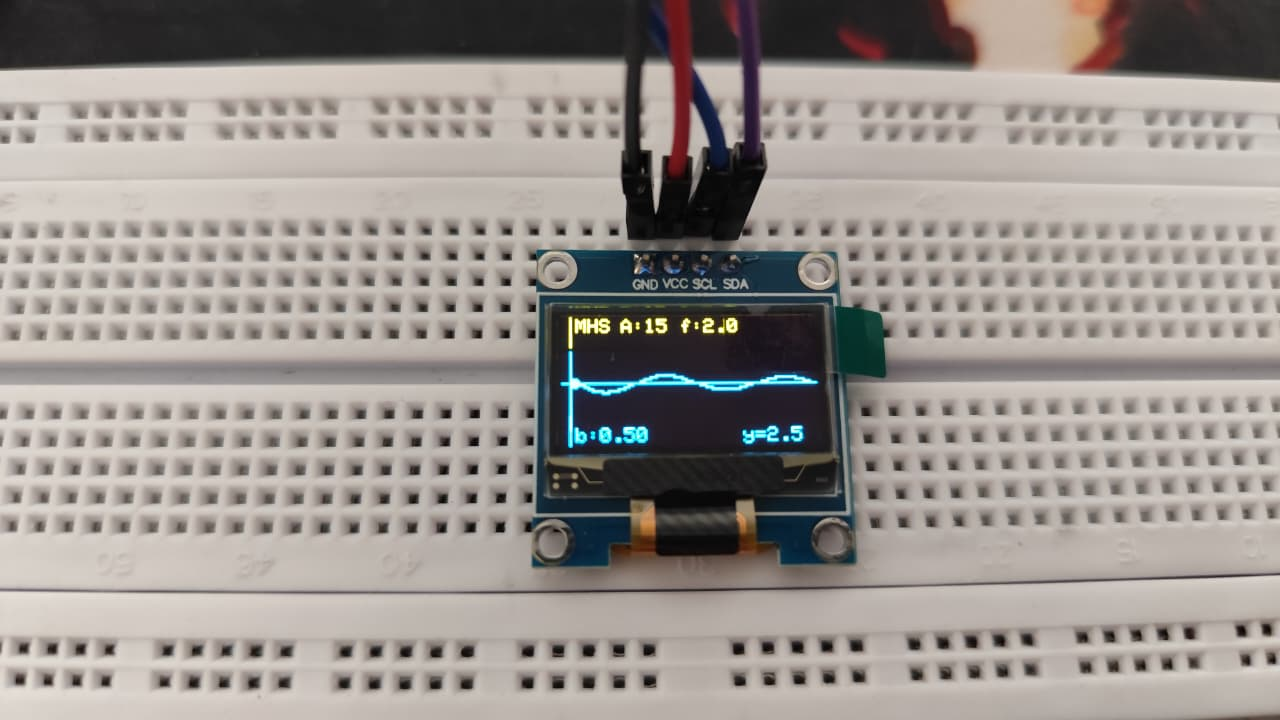
\includegraphics[width=\textwidth]{../Imagenes/Armonico_imgs/Armonico_img4.jpeg}
    \caption{Amortiguamiento avanzado ($\beta=0.50$): la onda casi se ha extinguido completamente}
    \label{fig:onda_amort2}
\end{subfigure}
\caption{Demostración del amortiguamiento: la envolvente $A e^{-\beta t}$ reduce progresivamente la amplitud}
\label{fig:amortiguamiento}
\end{figure}

\subsection{Interacción por Monitor Serial}

\begin{figure}[H]
\centering
\begin{subfigure}[b]{0.48\textwidth}
    \centering
    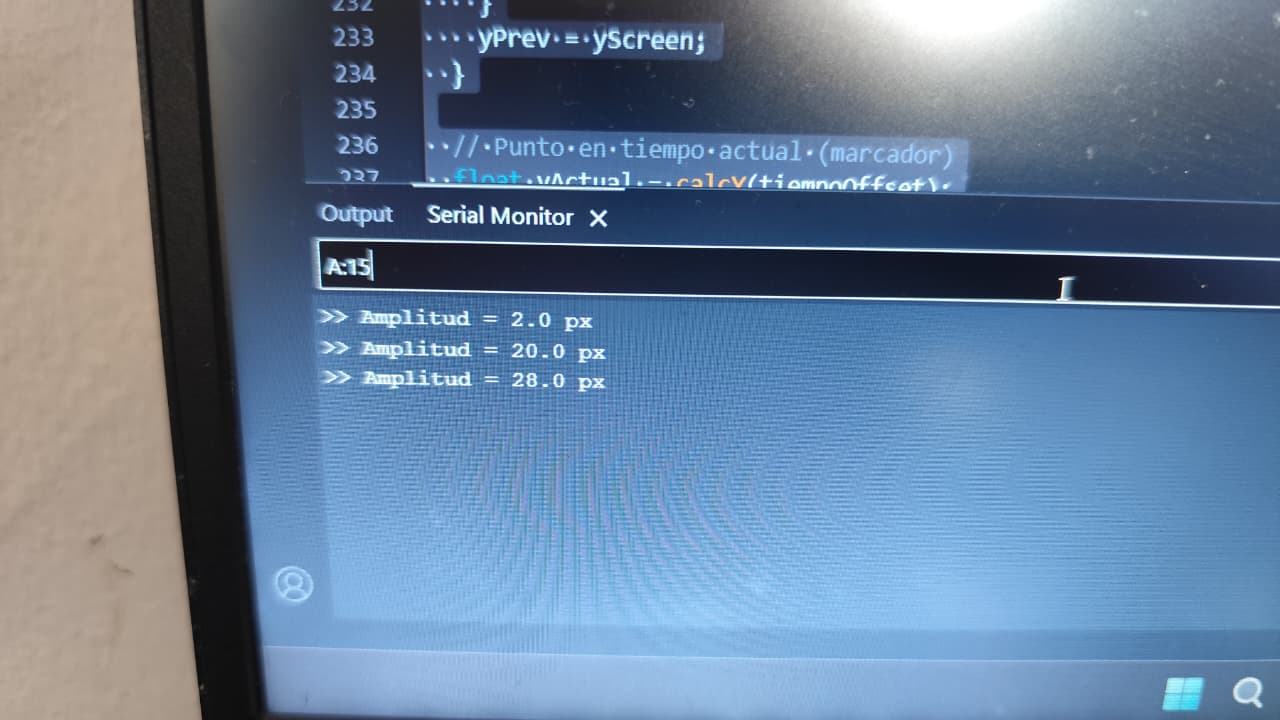
\includegraphics[width=\textwidth]{../Imagenes/Armonico_imgs/Armonico_img12.jpeg}
    \caption{Comando \texttt{A:15}: cambiando la amplitud a 15 píxeles}
    \label{fig:serial_amp}
\end{subfigure}
\hfill
\begin{subfigure}[b]{0.48\textwidth}
    \centering
    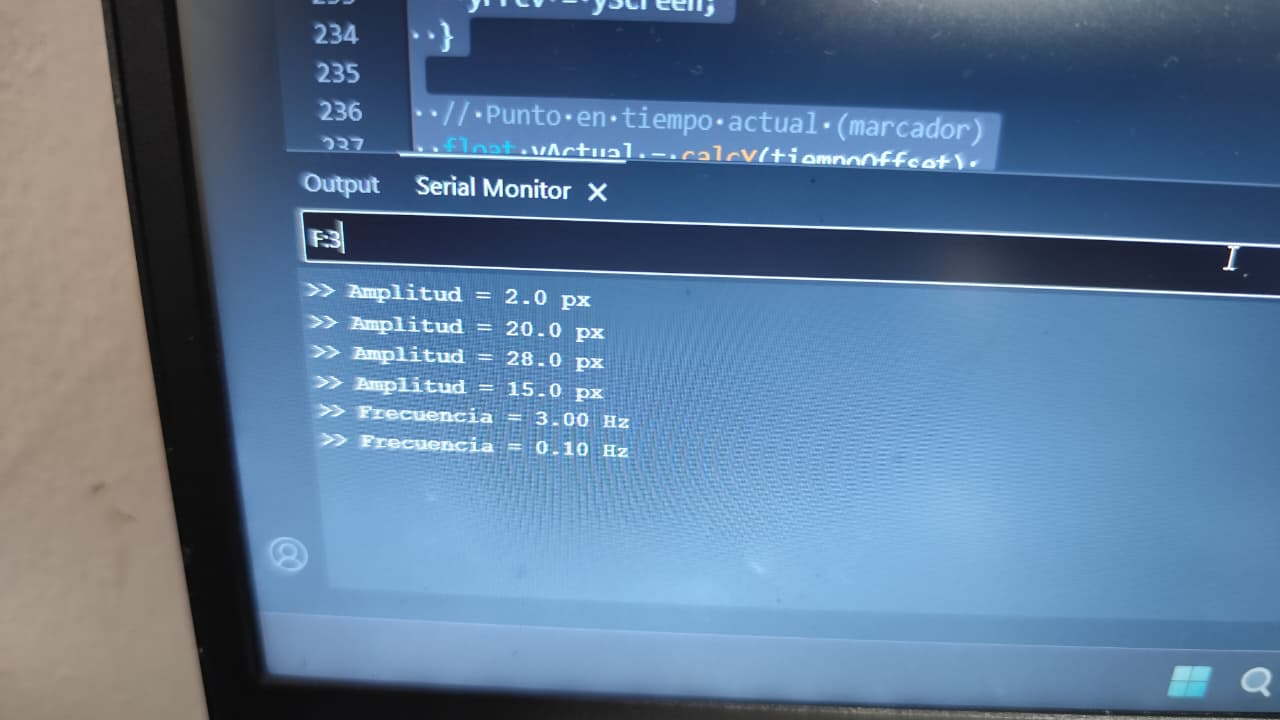
\includegraphics[width=\textwidth]{../Imagenes/Armonico_imgs/Armonico_img10.jpeg}
    \caption{Comando \texttt{F:3}: cambiando la frecuencia a 3\,Hz}
    \label{fig:serial_freq}
\end{subfigure}
\caption{Interacción con el Monitor Serial del Arduino IDE para modificar parámetros}
\label{fig:serial_params}
\end{figure}

\begin{figure}[H]
\centering
\begin{subfigure}[b]{0.48\textwidth}
    \centering
    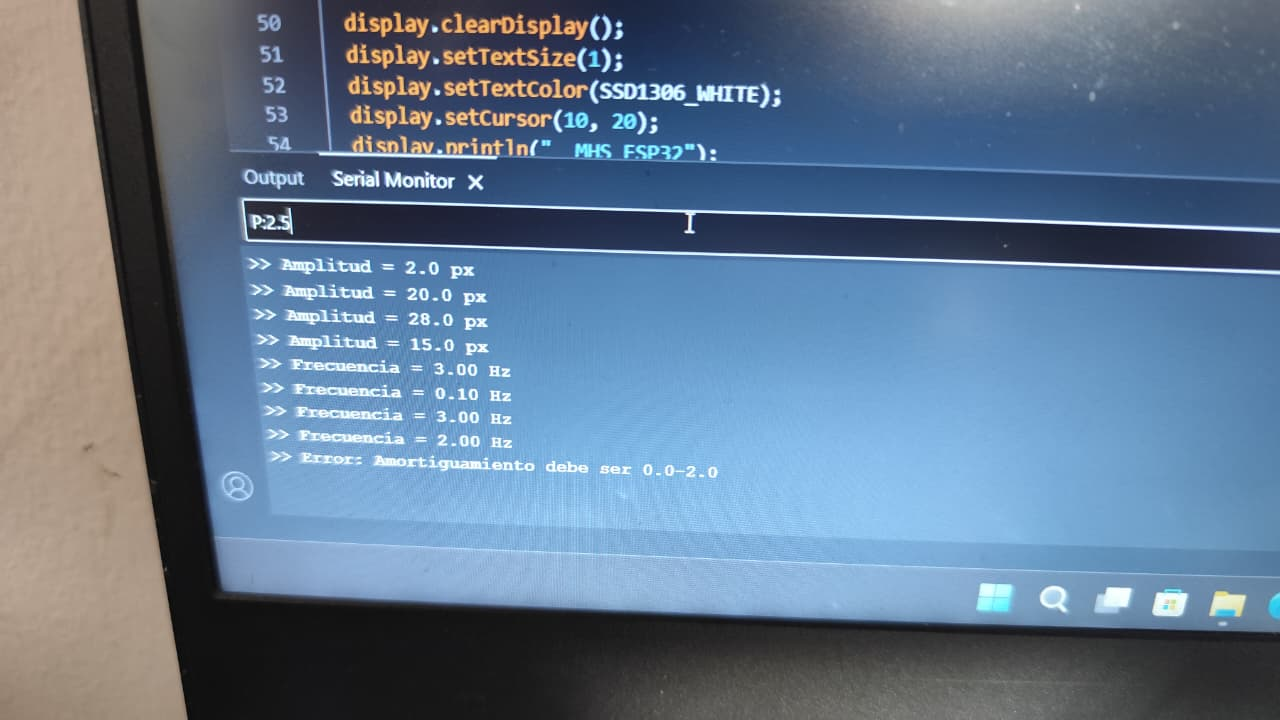
\includegraphics[width=\textwidth]{../Imagenes/Armonico_imgs/Armonico_img8.jpeg}
    \caption{Comando \texttt{P:2.5}: ajustando la fase inicial a 2.5\,rad}
    \label{fig:serial_fase}
\end{subfigure}
\hfill
\begin{subfigure}[b]{0.48\textwidth}
    \centering
    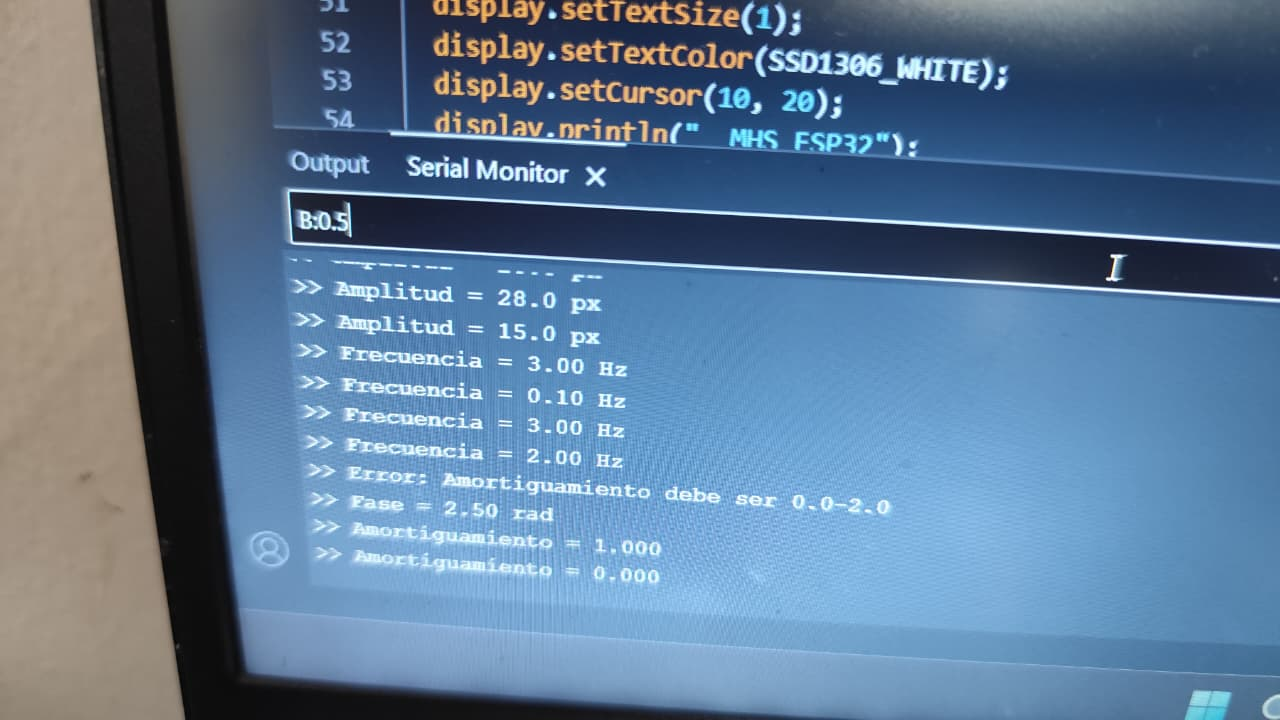
\includegraphics[width=\textwidth]{../Imagenes/Armonico_imgs/Armonico_img6.jpeg}
    \caption{Comando \texttt{B:0.5}: activando el amortiguamiento}
    \label{fig:serial_amort}
\end{subfigure}
\caption{Ajuste de fase y amortiguamiento mediante comandos seriales}
\label{fig:serial_avanzados}
\end{figure}

\begin{figure}[H]
\centering
\begin{subfigure}[b]{0.48\textwidth}
    \centering
    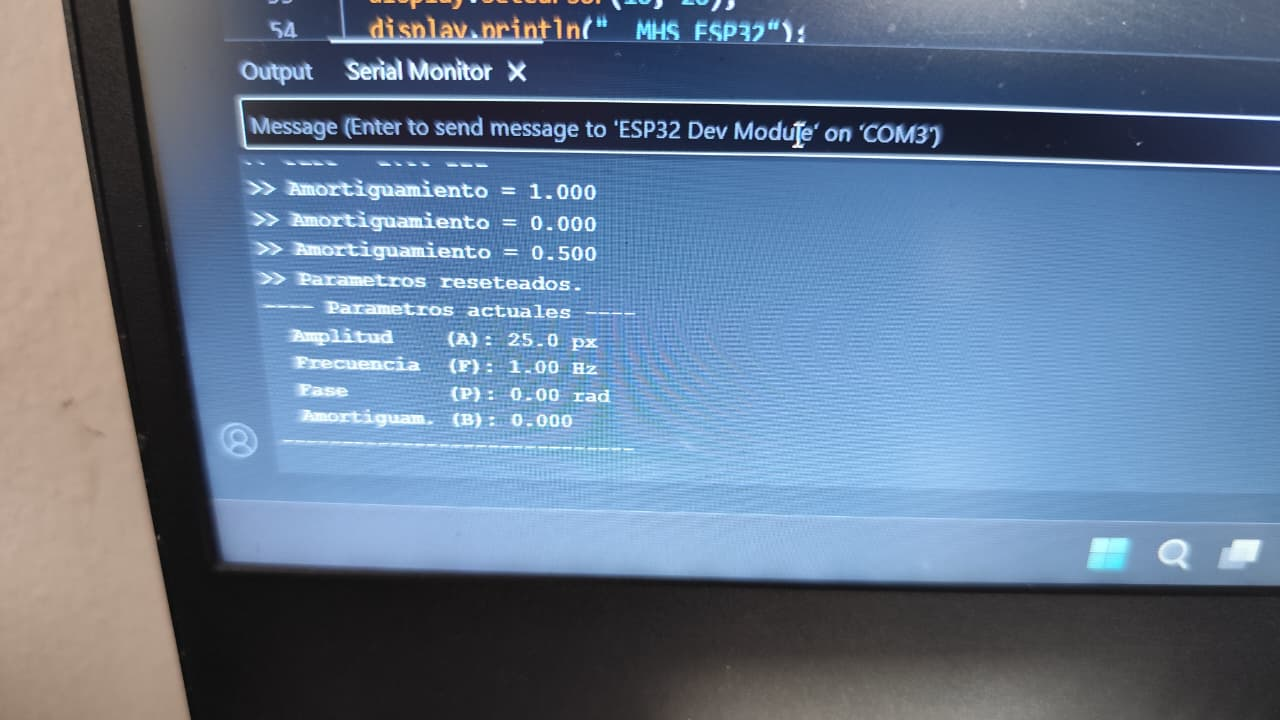
\includegraphics[width=\textwidth]{../Imagenes/Armonico_imgs/Armonico_img1.jpeg}
    \caption{Comando \texttt{R} y \texttt{?}: reset de parámetros y consulta de valores actuales}
    \label{fig:serial_reset}
\end{subfigure}
\hfill
\begin{subfigure}[b]{0.48\textwidth}
    \centering
    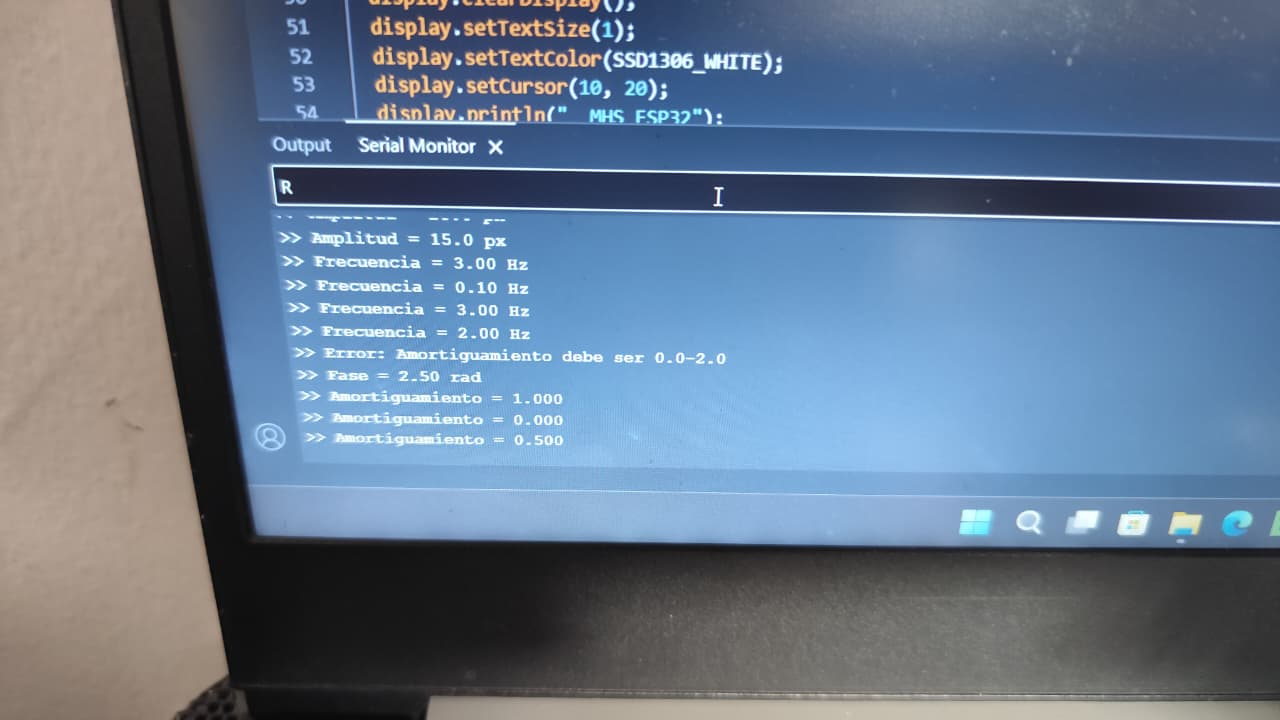
\includegraphics[width=\textwidth]{../Imagenes/Armonico_imgs/Armonico_img3.jpeg}
    \caption{Historial de comandos mostrando cambios sucesivos de múltiples parámetros}
    \label{fig:serial_hist}
\end{subfigure}
\caption{Funciones de reset, consulta y secuencia de comandos en el Monitor Serial}
\label{fig:serial_util}
\end{figure}

% ══════════════════════════════════════════════════════════════
\section{Proceso de Creación}
% ══════════════════════════════════════════════════════════════

\begin{enumerate}
    \item \textbf{Selección de componentes:} Se eligió la pantalla OLED SSD1306 de 0.96'' por su bajo consumo, alto contraste y compatibilidad I2C con solo 4 cables de conexión.

    \item \textbf{Diseño del circuito:} Se diseñó el esquema en Fritzing (Figura~\ref{fig:esquema}), conectando los pines I2C de la OLED (SDA, SCL) a GPIO21 y GPIO22 del ESP32 respectivamente, con alimentación desde el pin de 3.3V.

    \item \textbf{Montaje en protoboard:} Se insertó la pantalla OLED en la protoboard y se conectó al ESP32 (montado en su placa de expansión con borneras) mediante 4 cables jumper.

    \item \textbf{Programación:} Se desarrolló el firmware con la siguiente arquitectura:
    \begin{itemize}
        \item Módulo matemático: función \texttt{calcY(t)} implementando la ecuación del MHS amortiguado.
        \item Módulo gráfico: función \texttt{dibujarGrafica()} para renderizado a 30 FPS.
        \item Módulo de interfaz: función \texttt{procesarSerial()} como parser de comandos.
    \end{itemize}

    \item \textbf{Configuración del Arduino IDE:}
    \begin{itemize}
        \item Placa: \textit{ESP32 Dev Module}.
        \item Librerías instaladas: Adafruit SSD1306, Adafruit GFX.
        \item Velocidad serial: 115200 baudios.
    \end{itemize}

    \item \textbf{Pruebas:} Se verificó el correcto funcionamiento variando cada parámetro individualmente y observando el efecto en la pantalla OLED y el Monitor Serial.
\end{enumerate}

% ══════════════════════════════════════════════════════════════
\section{Conclusiones}
% ══════════════════════════════════════════════════════════════

\begin{itemize}
    \item El proyecto demuestra la simulación visual de un fenómeno físico fundamental (MHS) sobre hardware embebido de bajo costo, logrando una representación gráfica fluida a 30 FPS.
    \item La implementación directa de la ecuación $y(t) = A e^{-\beta t} \sin(2\pi f t + \varphi)$ permite observar en tiempo real el efecto de cada parámetro sobre la forma de onda.
    \item La interfaz serial interactiva con comandos \texttt{A:}, \texttt{F:}, \texttt{P:} y \texttt{B:} proporciona una herramienta pedagógica eficaz para explorar la física de las oscilaciones.
    \item El protocolo I2C demostró ser ideal para esta aplicación, requiriendo únicamente 2 líneas de datos (más alimentación) para controlar un display gráfico completo.
    \item La técnica de renderizado punto a punto con interpolación vertical entre píxeles consecutivos produce curvas suaves a pesar de la baja resolución (128$\times$64).
    \item El uso de la función \texttt{constrain()} para limitar las coordenadas de pantalla evita escrituras fuera del buffer, una práctica esencial en programación de displays.
    \item Este proyecto sienta las bases para aplicaciones más avanzadas como osciloscopios digitales, analizadores de espectro o simuladores de circuitos RLC en pantallas embebidas.
\end{itemize}

\end{document}
